\subparagraph*{Submission : }
\textit{Consider the general case in which the shop needs to optimize the prices and the assignment of promos to the customers in the case all the parameters need to be learnt.}\\

The problem requires to find the optimal prices for the two items and to optimize the assignment of the promos, in the scenario where all the parameters need to be learnt.

Implementation: \textit{n6.py}
\subsection*{Strategy}
We simulate the random arrival of the customers. We have used a TS learner, with a number of arms equal to by the product between the number of pricing candidates for the first item and the number of pricing candidates of the second item. We pull the learner to retrieve a superarm, that specifies the couple of prices of the two items. For each possible superarm we have a Promo-Category UCB learner that is used to learn the promo-category assignment that maximize the reward.  We evaluate, for each customer, the purchase of the first item at the suggested price. In case that the customer buys the first item, using the Promo-Category UCB learner associated with the superarm, we pull the optimal matching and we propose to the client the second item at the discounted price, according to the category he belongs to. Before the arrival of a new customer, we update the TS learner with the entire reward given by the two items, and the UCB learner with the reward of the second item. We have used the same two matrixes, in the same way of the previous request.

\subparagraph{Implementation} 
\begin{itemize}
	\item No seasonality, conversion rate do no change
	\item Number of customers per class is not known 
	\item Candidates for the \textit{Racing Skis} are: \{2110.0, 1900.0, 2420.0, 2690.00\}
	\item Candidates for the \textit{Racing Ski Helmet} are: \{360.0, 410.0, 530.0, 600.0\}
	\item Conversion rate associated with the first item is not known
	\item Conversion rate associated with the second item is not known
	\item Promotion assignment is not known 
\end{itemize}


\subparagraph{Optimal strategy}
In order to calculate the regret, we have defined the optimal solution calculation in the following manner, using an offline approach. We calculate the maximum achievable reward choosing all the possible configuration of prices for the two items.We compute the reward achievable for every couple of candidates as the sum of the achievable reward of the two items, taking into account that the sold of the second item is limited by the number of the customers that by also the first one. 
According to our candidates the optimal solution is:
\begin{center}
	\begin{tabular}{|c|p{4cm}|p{4cm}|p{4cm}|} 
	\hline
	Season & \textit{Racing Skis optimal price} & \textit{Racing Ski Helmet} optimal price & Optimal promo-category matching \\ \hline
	\multirow{4}{*}{Spring-Summer} & \multirow{4}{*}{1900.0} & \multirow{4}{*}{410.0} & Sport addicted: P$_0$ = 0\% (410.0)  \\ 
								   & 					   &                      & Gifted: P$_2$ = 20\% (328.0)          \\ 
								   & 					   &                      & Worried: P$_3$ = 30\% (287.0)         \\
								   & 					   &                      & Amateur: P$_1$ = 10\% (369.0)         \\ \hline
	\end{tabular}
\end{center}

\subsection*{Results}
\begin{center}
	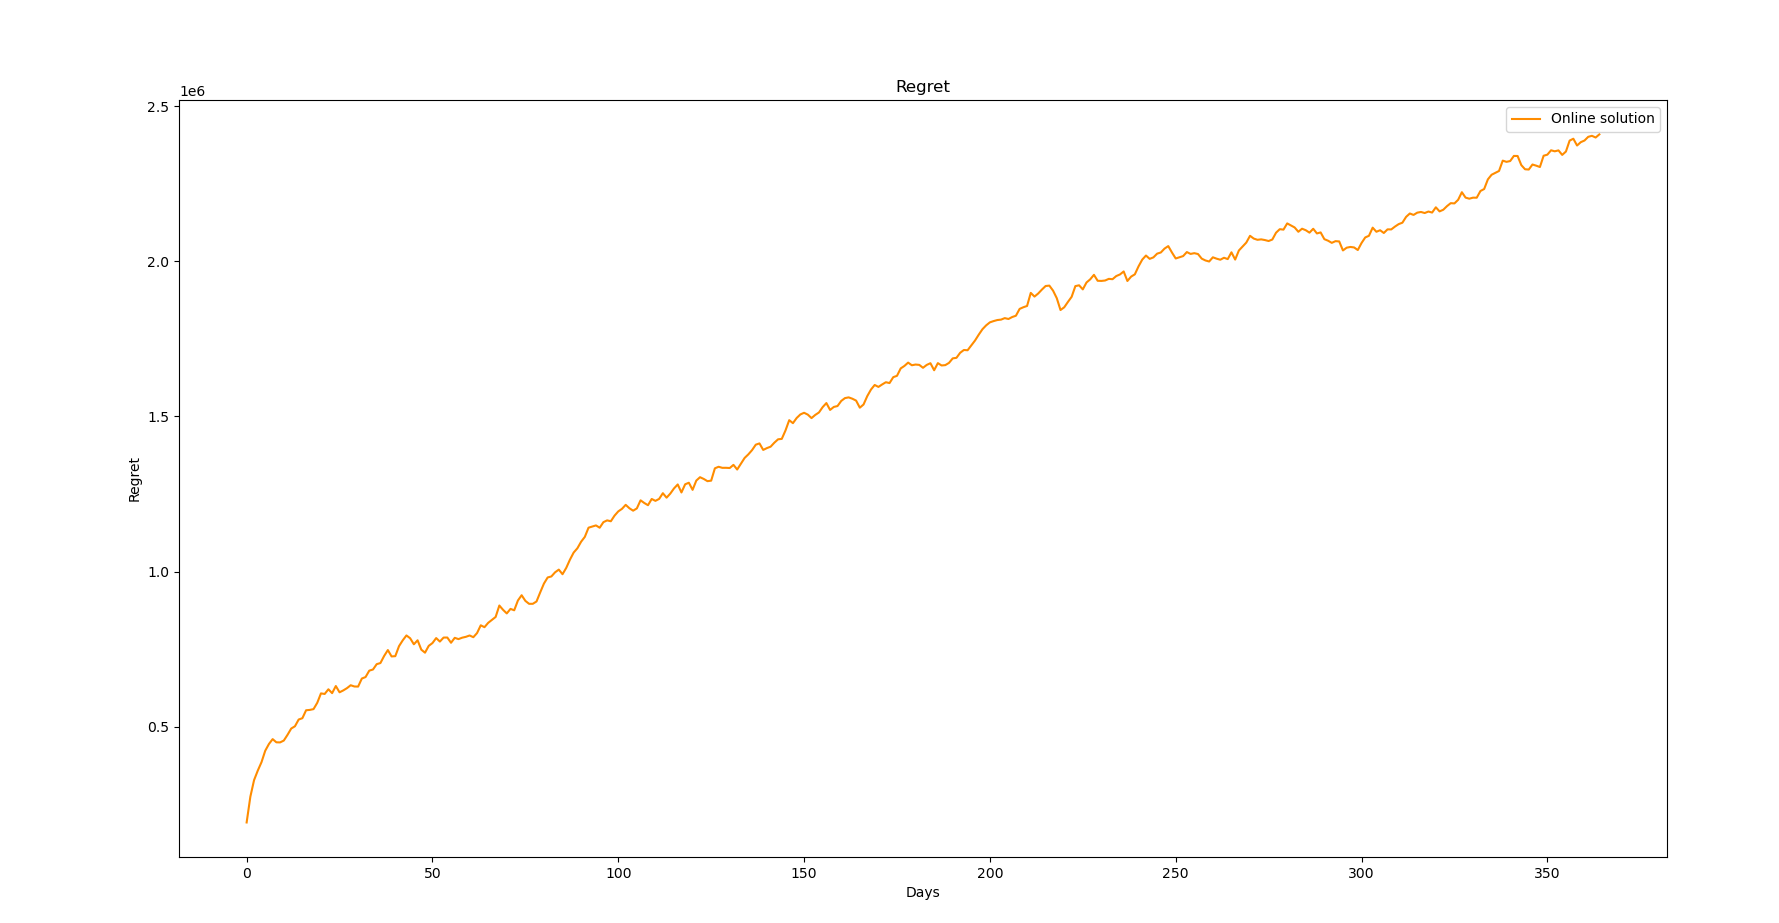
\includegraphics[scale=0.35]{Images/n6}
\end{center}
Days: 365\\
Experiments number: 3 \\
Starting delay of the Promo-Category UCB Matching: 1000 clients\\

\subsection*{Considerations}
We can notice that the learners take more time to learn the optimal solutions for both pricing and matching. The cumulative regret is increasing quite linearly up to the middle of the time horizon, after that, they start to stabilize on the optimal solutions. The cumulative regret still be jagged, because the performance of the matching are worst compared to the pricing, morehover we have to take in consideration that the choice of the first item price impact on the performance of the second item (an unattractive price for the first item decrease the number of samples usable for the second price learning).